\documentclass[12pt]{extreport} % Schriftgröße: 8pt, 9pt, 10pt, 11pt, 12pt, 14pt, 17pt oder 20pt

%% Packages
\usepackage{scrextend}
\usepackage{amssymb}
\usepackage{amsthm}
\usepackage{booktabs}
\usepackage{caption}
\usepackage{subcaption}
\usepackage{chngcntr}
\usepackage{cmap}
\usepackage{color}
\usepackage{csquotes}
\usepackage{enumitem}
\usepackage{float}
\usepackage{graphicx}
\usepackage{hyperref}
\usepackage{underscore}
\usepackage{ulem}
\usepackage{lmodern}
\usepackage{makeidx}
\usepackage{amsmath}
\usepackage{mathtools}
\usepackage{xpatch}
\usepackage{pgfplots}
\pgfplotsset{compat=1.12}
\usepgfplotslibrary{fillbetween}
\usepackage{amsfonts}
\usetikzlibrary{calc}	
\usetikzlibrary{matrix}	
\usepackage{fancyhdr}
\usepackage{epstopdf}

% Language Setup 
\usepackage[utf8]{inputenc} 
\usepackage[T1]{fontenc} 
\usepackage[ngerman]{babel}

% Options
\makeatletter%%  
  % Linkfarbe, {0,0.35,0.35} für Türkis, {0,0,0} für Schwarz, {1,0,0} für Rot, {0,0,0.85} für Blau
  \definecolor{linkcolor}{rgb}{0,0.35,0.35}
  % Zeilenabstand für bessere Leserlichkeit
  \def\mystretch{1.2} 
  % Publisher definieren
  \newcommand\publishers[1]{\newcommand\@publishers{#1}} 
  % Enumerate im 1. Level: \alph für a), b), ...
  \renewcommand{\labelenumi}{\alph{enumi})} 
  % Enumerate im 2. Level: \roman für (i), (ii), ...
  \renewcommand{\labelenumii}{(\roman{enumii})}
  % Zeileneinrückung am Anfang des Absatzes
  \setlength{\parindent}{0pt} 
  % Für das Proof-Environment: 'Beweis:' anstatt 'Beweis.'
  \xpatchcmd{\proof}{\@addpunct{.}}{\@addpunct{:}}{}{} 
  % Nummerierung der Bilder, z.B.: Abbildung 4.1
  \@ifundefined{thechapter}{}{\def\thefigure{\thechapter.\arabic{figure}}} 
  % Chapter-Nummerierung beginnen bei (0):
  \setcounter{chapter}{0}
  % Chapter-Nummerierung
  \renewcommand\thechapter{\Roman{chapter}}
\makeatother%

% Meta Setup 
\title{Globale Optimierung - Sonderübung IV}
\author{Kostorz, Belica}
\date{Sommersemester 2017}
\publishers{Karlsruher Institut für Technologie}

\fancypagestyle{firststyle}
{
   \fancyhf[C]{\small Globale Optimierung - Sonderübung IV ~\\ Nadine Kostorz (1972005), Leon Talenberg (1957966), Martin Belica (1775706)}
   \fancyfoot[C]{}
}

%% Math. Definitiones
\newcommand{\C}{\mathbb{C}}
\newcommand{\N}{\mathbb{N}}
\newcommand{\Q}{\mathbb{Q}}
\newcommand{\R}{\mathbb{R}}
\newcommand{\Z}{\mathbb{Z}}
\newcommand{\DO}[1]{\mathcal{D}\left( {#1} \right)}
\newcommand{\RO}[1]{\mathcal{R}\left( {#1} \right)}

%% Template
\makeatletter%
\DeclareUnicodeCharacter{00A0}{ } \pgfplotsset{compat=1.7} \hypersetup{colorlinks,breaklinks, urlcolor=linkcolor, linkcolor=linkcolor, pdftitle=\@title, pdfauthor=\@author, pdfsubject=\@title, pdfcreator=\@publishers}\DeclareOption*{\PassOptionsToClass{\CurrentOption}{report}} \ProcessOptions \def\baselinestretch{\mystretch} \setlength{\oddsidemargin}{0.125in} \setlength{\evensidemargin}{0.125in} \setlength{\topmargin}{0.5in} \setlength{\textwidth}{6.25in} \setlength{\textheight}{8in} \addtolength{\topmargin}{-\headheight} \addtolength{\topmargin}{-\headsep} \def\pulldownheader{ \addtolength{\topmargin}{\headheight} \addtolength{\topmargin}{\headsep} \addtolength{\textheight}{-\headheight} \addtolength{\textheight}{-\headsep} } \def\pullupfooter{ \addtolength{\textheight}{-\footskip} } \def\ps@headings{\let\@mkboth\markboth \def\@oddfoot{} \def\@evenfoot{} \def\@oddhead{\hbox {}\sl \rightmark \hfil \rm\thepage} \def\chaptermark##1{\markright {\uppercase{\ifnum \c@secnumdepth >\m@ne \@chapapp\ \thechapter. \ \fi ##1}}} \pulldownheader } \def\ps@myheadings{\let\@mkboth\@gobbletwo \def\@oddfoot{} \def\@evenfoot{} \def\sectionmark##1{} \def\subsectionmark##1{}  \def\@evenhead{\rm \thepage\hfil\sl\leftmark\hbox {}} \def\@oddhead{\hbox{}\sl\rightmark \hfil \rm\thepage} \pulldownheader }	\def\chapter{\cleardoublepage  \thispagestyle{plain} \global\@topnum\z@ \@afterindentfalse \secdef\@chapter\@schapter} \def\@makeschapterhead#1{ {\parindent \z@ \raggedright \normalfont \interlinepenalty\@M \Huge \bfseries  #1\par\nobreak \vskip 40\p@ }} \newcommand{\indexsection}{chapter} \patchcmd{\@makechapterhead}{\vspace*{50\p@}}{}{}{}\def\Xint#1{\mathchoice
    {\XXint\displaystyle\textstyle{#1}} {\XXint\textstyle\scriptstyle{#1}} {\XXint\scriptstyle\scriptscriptstyle{#1}} {\XXint\scriptscriptstyle\scriptscriptstyle{#1}} \!\int} \def\XXint#1#2#3{{\setbox0=\hbox{$#1{#2#3}{\int}$} \vcenter{\hbox{$#2#3$}}\kern-.5\wd0}} \def\dashint{\Xint-} \def\Yint#1{\mathchoice {\YYint\displaystyle\textstyle{#1}} {\YYYint\textstyle\scriptscriptstyle{#1}} {}{} \!\int} \def\YYint#1#2#3{{\setbox0=\hbox{$#1{#2#3}{\int}$} \lower1ex\hbox{$#2#3$}\kern-.46\wd0}} \def\YYYint#1#2#3{{\setbox0=\hbox{$#1{#2#3}{\int}$}  \lower0.35ex\hbox{$#2#3$}\kern-.48\wd0}} \def\lowdashint{\Yint-} \def\Zint#1{\mathchoice {\ZZint\displaystyle\textstyle{#1}}{\ZZZint\textstyle\scriptscriptstyle{#1}} {}{} \!\int} \def\ZZint#1#2#3{{\setbox0=\hbox{$#1{#2#3}{\int}$}\raise1.15ex\hbox{$#2#3$}\kern-.57\wd0}} \def\ZZZint#1#2#3{{\setbox0=\hbox{$#1{#2#3}{\int}$} \raise0.85ex\hbox{$#2#3$}\kern-.53\wd0}} \def\highdashint{\Zint-} \DeclareRobustCommand*{\onlyattoc}[1]{} \newcommand*{\activateonlyattoc}{ \DeclareRobustCommand*{\onlyattoc}[1]{##1} } \AtBeginDocument{\addtocontents{toc} {\protect\activateonlyattoc}} \newcommand{\RightArrow}{\xRightarrow[]{ ~ ~ }} \newcommand{\LeftArrow}{\xLeftarrow[]{ ~ ~ }} \newcommand{\rightArrow}{\xrightarrow[]{ ~ ~ }} \newcommand{\leftArrow}{\xleftarrow[]{ ~ ~ }}
	% Titlepage
	\def\maketitle{ \begin{titlepage} 
			~\vspace{3cm} 
		\begin{center} {\Huge \@title} \end{center} 
	 		\vspace*{1cm} 
	 	\begin{center} {\large \@author} \end{center} 
	 	\vspace*{-0.5cm}
	 	\begin{center} \@date \end{center} 
	 		\vspace*{7cm} 
	 	\begin{center} \@publishers \end{center} 
	 		\vfill 
	\end{titlepage} }
\makeatother%

% Create Index
\makeindex 

\begin{document}

\thispagestyle{empty}
\pagenumbering{arabic}\thispagestyle{firststyle}

\subsubsection*{Aufgabe 1}

\begin{enumerate}
	\item Berechnen Sie die Hessematrix $D^2f$ der Funktion
		$$ f(x) = x^2_1 x_2 + 2 x_1 x_2^2 + x_1 x_2. $$ 
		\begin{proof}
			Da $f$ als Polynom in $C^2$ liegt, folgt:
			$$ \nabla f(x) = \begin{pmatrix} 2 x_1 x_2 + 2 x_2^2 + x_2 \\ x_1^2 + 4 x_1 x_2 + x_1 \end{pmatrix} \text{ und damit } D^2 f(x) = \begin{pmatrix}
				2 x_2 & 2 x_1 + 4x_2 + 1 \\ 2 x_1 + 4x_2 + 1 & 4 x_1
			\end{pmatrix} $$
		\end{proof}
	\item Implementieren Sie eine Funktion $DsqF(X)$, die zu gegebenem Interval $X \in \mathbb{IR}^2$ die (eintragsweise) natürliche Intervallerweiterung $D^2F$ von $D^2f$ zurück gibt. \smallskip
	
		$DsqF$ soll ein $(2, 2, 2)$-Array zurück geben, deren Einträge $(i, j, 1)$ die Unter- und $(i, j, 2)$ die Obergrenze von $F_{i,j}(X)$ enthalten, $i, j \in \{1, 2\}$. Die Box $X$ soll als $(2,2)$-Array übergeben werden, deren Einträge $(i, 1)$ die Untergrenze $\underline{x}_i$ und $(i, 2)$ die Obergrenze $\overline{x}_i$, $i \in \{1, \dotsc, n \}$ der jeweiligen Intervalle enthalten. Nutzen Sie für die Grundrechenarten der Intervallarithmetik die Funktionen aus Aufgabe S. 3.2.
			\begin{figure*}[h!] \centering
				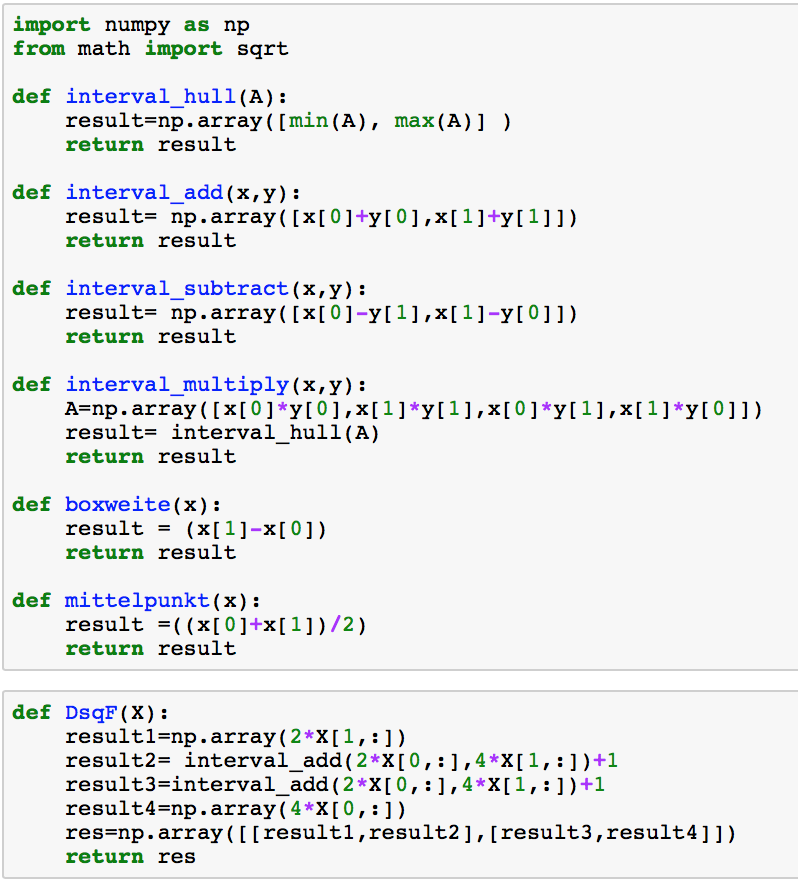
\includegraphics[scale=.525]{img/su2iv-i}
			\end{figure*}
\end{enumerate}
 
\newpage

\subsubsection*{Aufgabe 2}


Es seien $A(x) = D^2f(x)$ die $(n,n)$-Hessematrix einer Funktion $f$ und alle Einträge $a_{ij}$ faktorisierbar. Für eine Box $X \in \mathbb{IR}^n$ bezeichne $A(X)$ diejenige Matrix, deren Einträge $A_{ij}$ natürliche Intervallerweiterung von $a_{ij}$ sind. ~\smallskip

Implementieren Sie eine Funktion $lambda$_$min$ die für eine Box $X$ und die Matrix $A(X)$ eine Unterschranke $\beta$ des kleinsten Eigenwertes $\lambda_{\min}(D^2f(x))$ auf $X$ berechnet. Verwenden sie hierfür die Formel aus Skript S. 146. ~\smallskip

Die intervallwertige Hessematrix $A$ soll dabei als $(n,n,2)$-Array übergeben werden, deren Einträge $(i,j,1)$ die Unter- und $(i,j,2)$ die Obergrenze von $F_{i,j}(X)$ enthalten, $i,j \in \{1, \dotsc, n\}$. Die Box $X$ soll als $(n, 2)$-Array übergeben werden, deren Einträge $(i, 1)$ die Untergrenze $\underline{x}_i$ und $(i, 2)$ die Obergrenze $\overline{x}_i$, $i \in \{1, \dotsc, n \}$ der jeweiligen Intervalle enthalten.

			\begin{figure*}[h!] \centering
				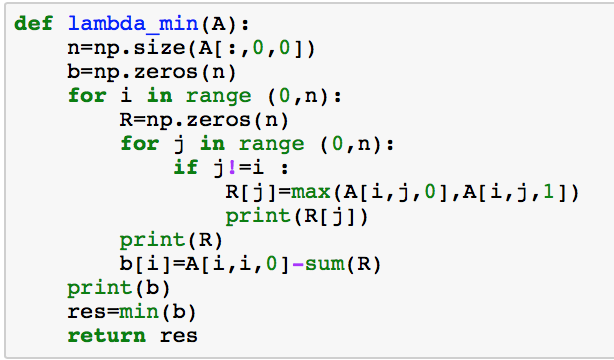
\includegraphics[scale=.75]{img/su2iv-ii}
			\end{figure*}
\newpage

\subsubsection*{Aufgabe 3}

Betrachten Sie nun wieder die Funktion
	$$ f(x) = x_12 x_2 + 2x_1 x_2^2 + x_1 x_2 $$
auf der Box $X = [0, 1] \times [-1, 1]$.

\begin{enumerate}
	\item Nutzen Sie Ihre in Aufgabe S. 4.1. implementierte Funktion, um die Matrix $D^2 F(X)$ auszugeben. Verwenden Sie Ihre in Aufgabe 4.2 implementierte Fkt. $lambda$_$min$, um eine Unterschranke $\beta$ des kleinsten Eigenwertes der Hessematrix $D^2 f$ auf $X$ zu berechnen und geben Sie diese aus.
		\begin{proof} ~\\
			\begin{figure*}[h!] \centering
				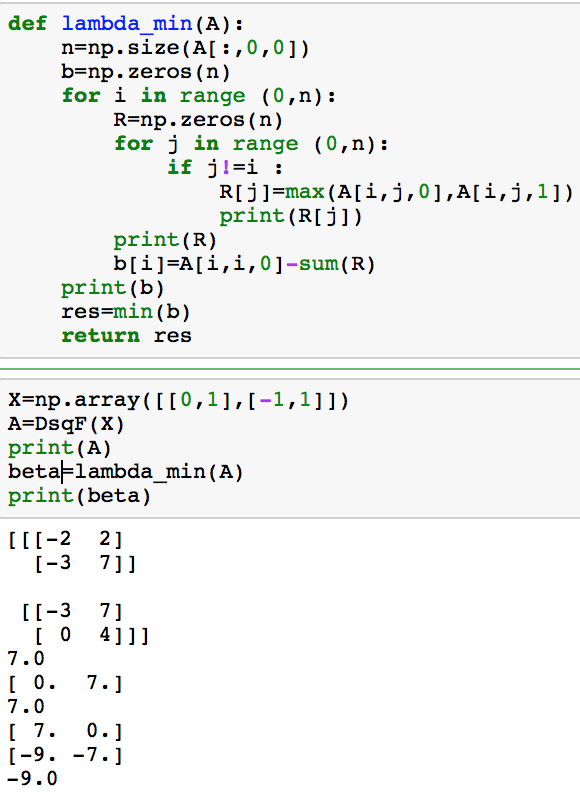
\includegraphics[scale=0.7]{img/su2iv-iii-1}
			\end{figure*}
		\end{proof} \newpage
	\item Bestimmen Sie mit Hilfe von Aufgabenteil a) eine konvexe Relaxierung $\hat{f}_\alpha$ der Funktion $f$ auf $X$. Geben Sie diese auf der schriftlichen Abgabe an.
		\begin{proof}
			$$ \hat{f}_\alpha = x_1^2 x_2 + 2 x_1 x_2^2 + x_1 x_2 + \frac{9}{2} \left( - x_1 + x_1^2 + x_2^2 -1 \right) $$
		\end{proof}
	\item Plotten Sie die beiden Funktionen $\hat{f}_\alpha$ und $f$ auf $X$ in eine Grafik, sodass gut erkennbar ist, dass $\hat{f}_\alpha$ konvexe Relaxierung von $f$ auf $X$ ist.
		\begin{proof} ~\\
			\begin{figure*}[h!] \centering
				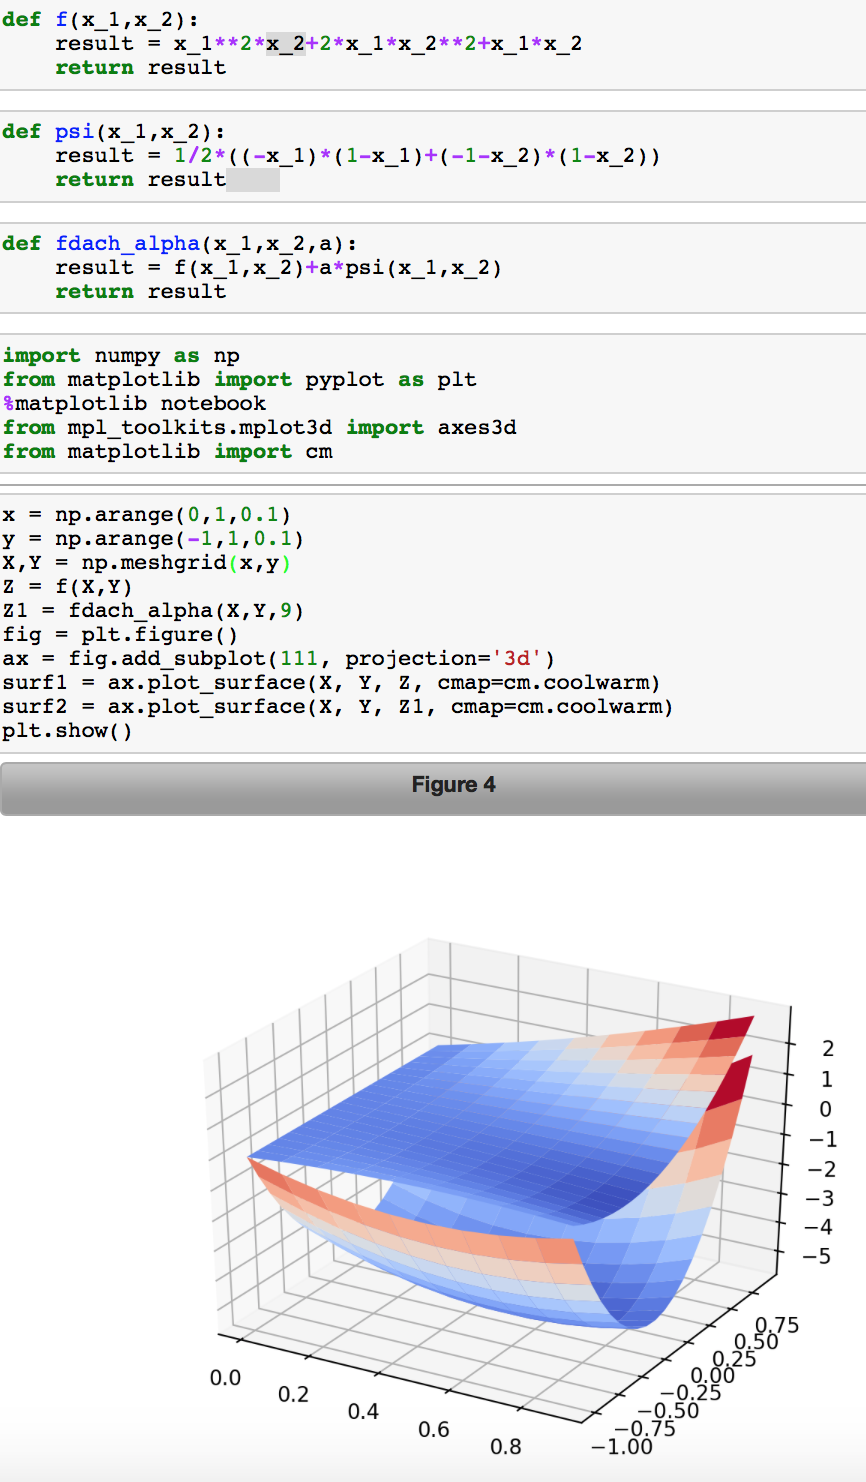
\includegraphics[scale=0.46]{img/su2iv-iii-2}
			\end{figure*}
		\end{proof} \newpage
	\item Welche Teilboxen $X^1$ und $X^2$ ergeben sich, wenn die Box entsprechend Algorithmus 3.3 halbiert wird? Mit der Notation von Algorithmus 3.3: Plotten Sie $f$ auf $X$, $\hat{f}_{\alpha}^1$ auf $X^1$ und $\hat{f}_{\alpha}^2$ auf $X^2$ in eine Grafik.
		\begin{proof}
			Nach Algorithmus 3.3 
			$$ X^1 = [0, 1] \times [-1, 0], \quad X^2 = [0, 1] \times [0, 1] $$
			
			\begin{figure*}[h!] \centering
				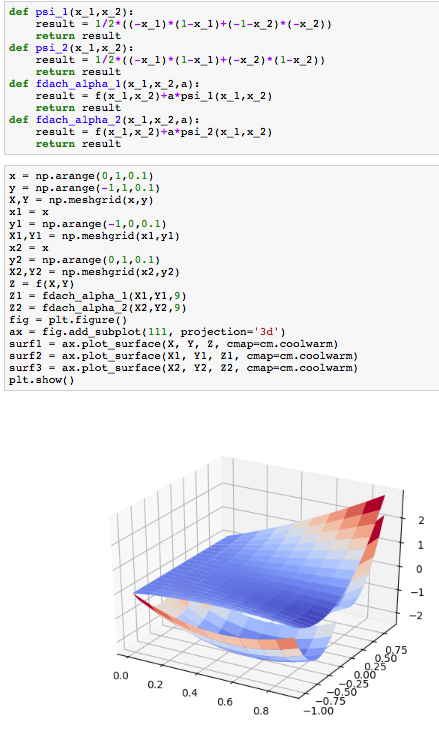
\includegraphics[scale=0.55]{img/su2iv-iii-3}
			\end{figure*}
		\end{proof}
	\item Bestimmen Sie nun mit der Funktion $lambda$_$min$ individuelle Unterschranken des kleinsten Eigenwertes der Hessematrix $D^2 f$ auf $X^i$, $i \in \{1, 2 \}$ und geben Sie diese aus. Nutzen Sie diese, um (möglicherweise) bessere Relaxierungen $\hat{f}^1_{\alpha_1}$ und $\hat{f}^2_{\alpha_2}$  zu bestimmen. Plotten Sie $f$ auf $X$, $\hat{f}^1_{\alpha_1}$ auf $X^1$ und $\hat{f}^2_{\alpha_2}$ auf $X^2$ in eine Grafik. Vergleichen Sie Ihr Ergebnis mit Aufgabenteil d).
			\begin{figure*}[h!] \centering
				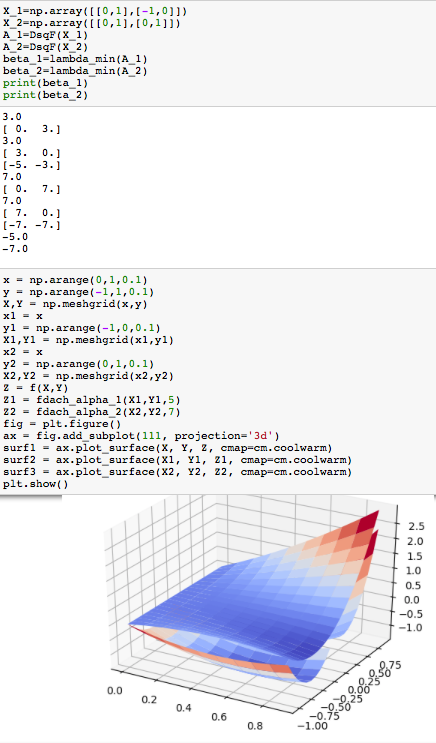
\includegraphics[scale=0.625]{img/su2iv-iii-4}
			\end{figure*}
	\item Bestimmen Sie Optimalpunkte von $\hat{f}^1_{\alpha_1}$ auf $X^1$ und $\hat{f}^2_{\alpha_2}$ auf $X^2$ mit einem Solver Ihrer Wahl. Runden Sie das Ergebnis auf zwei Nachkommastellen. Bestimmen Sie $\tilde{v}$ und $\hat{v}^*$? Begründen Sie: Würde $X^1$ oder $X^2$ als $X^*$ für die nächste Iteration von Algorithmus 3.3 verwendet werden?
		\begin{proof}
			Es ist $\hat{x}^1 \approx (0.26, -0.47)$, $\hat{x}^2 \approx (0.38, 0.35)$
			$$ \Rightarrow \tilde{x} = \hat{x}^1 $$
			$\tilde{v} = f(\hat{x}^1) \approx -0.1982$, $\hat{v}^* = \hat{f}_{\alpha_1}(\hat{x}^1) \approx -1.4099$
			$$ \Rightarrow x^* = x^1, \text{ da } \hat{v}^1 = \min_{l =1, 2} \hat{v}^l $$
			\begin{figure*}[h!] \centering
				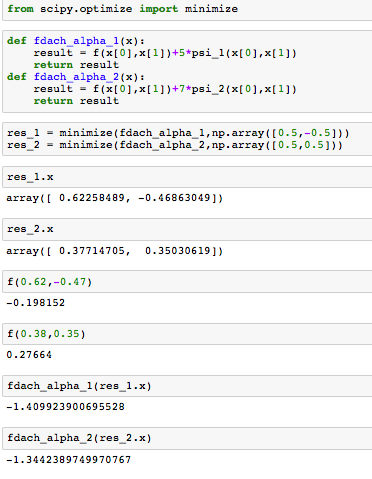
\includegraphics[scale=0.65]{img/su2iv-iii-5}
			\end{figure*}
		\end{proof} \newpage
	\item Bestimmen Sie, aufbauend auf Aufgabenteil f), ein möglichst kleines Intervall, in dem der optimale Zielfunktionswert $v$ liegt.
		\begin{proof}
			Es ist
			$$ -1.4099 \leq v \leq -0.1982 \iff v \in [-1.4099, -0.1982] $$
		\end{proof}
	\item Was passiert, wenn Sie versuchen mit dem in Aufgabenteil d) verwendeten Solver das Minimum von $f$ auf$ X$ mit Startpunkt $x_0 = (0,0)^T$ auszurechnen? Vergleichen Sie Ihr Ergebnis mit Aufgabenteil f) und g).
		\begin{proof}
			Mit dem Solver kommt als Minimalpunkt $x^* = (0, 0)$ raus, da 
			$$ f( (0,0) ) = 0 \notin [-1.4099, -0.1982], $$
			liegt der Optimalwert im Vergleich zu den vorherigen Aufgaben über der Oberschranke $\tilde{v} = -0.1982 \Rightarrow$ schlechteres Ergebnis.
		\end{proof}
\end{enumerate}

\newpage

\subsubsection*{Aufgabe 4}

Gegeben seien stetige Funktionen $f, g \colon X \rightarrow \R$, auf einer konvexen und kompakten Menge $X \subseteq \R^n$, die nicht notwendigerweise eine Box ist. Darüber hinaus sei $f$ nicht konvex und 
	$$ \hat{f} \coloneqq f + g $$
eine konvexe Relaxierung von $f$ auf $X$.

\textit{Sei o.B.d.A $X$ nicht-leer, dann sonst ist in den folgenden Teilaufgaben nichts zu zeigen.}	
	
\begin{enumerate}
	\item Folgt hieraus, dass $g$ eine konvexe Funktion ist? Beweisen Sie Ihre Behauptung.
		\begin{proof}
			Die gilt im Allgemeinen nicht. Betrachtet man den Fall $n = 2$ und $X = [-1, 1]^2$ (wodurch $X$ konvex ist), so folgt mit 
			$$ f(x) = \frac{1}{2} \left( 3 x_1^2 -  x_2^2 \right) ~ \text{ und } ~ \tilde{g}(x) = \frac{1}{2} \left( -x_1^2 + 3 x_2^2 \right), $$
			 dass $f$ und $g$ als Polynome in $C^1(X)$ liegen. Außerdem sind $f, g$ nicht konvex, was aus Satz 2.2.2 ($C^1$-Charakterisierung von Konvexität) folgt, da
			\begin{align*}
				f \left(\begin{pmatrix} 1 \\ 1 \end{pmatrix} \right) = 1 \leq & 1 + 2 = f \left(\begin{pmatrix} 1 \\ -1 \end{pmatrix} \right) + \left\langle \begin{pmatrix} 3 \\ 1 \end{pmatrix} ,  \begin{pmatrix} 1 \\ 1 \end{pmatrix} -  \begin{pmatrix} 1 \\ -1 \end{pmatrix} \right\rangle \\
				\tilde{g} \left(\begin{pmatrix} 1 \\ -1 \end{pmatrix} \right) = 1 \leq & 1 + 2 = \tilde{g} \left(\begin{pmatrix} -1 \\ -1 \end{pmatrix} \right) + \left\langle \begin{pmatrix} 1 \\ -3 \end{pmatrix} ,  \begin{pmatrix} 1 \\ -1 \end{pmatrix} -  \begin{pmatrix} -1 \\ -1 \end{pmatrix} \right\rangle \
			\end{align*} 
			Es gilt außerdem, dass
			$$ \frac{3}{2} x_1^2 \geq f(x) \geq -\frac{1}{2} x_2^2 $$
			für alle $x \in X$, sodass $f(x) \in [-0.5, 1.5]$ und analog $\tilde{g}(x) \in [-0.5, 1.5]$. Somit folgt mit $g \coloneqq g - 1.5$, dass als Verschiebung von $\tilde{g}$ die Funktion $g$ ebenfalls nicht konvex ist, $\hat{f}(x) = f(x) + g(x) = x_1^2 + x_2^2 - 1.5 \leq f(x)$ für alle $x \in X$. Außerdem ist $\hat{f}$ in $C^2(X)$ als Polynom und damit
			$$ D^2 \hat{f} = \begin{pmatrix}
				2 & 0 \\ 0 & 2
			\end{pmatrix} \succ 0 $$
			wodurch $\hat{f}$ nach Satz 2.5.3 ($C^2$-Charakterisierung von Konvexität) konvex ist. Insgesamt erhalten wir eine konvexe Funktion $\hat{f}$ für die $\hat{f}(x) \leq f(x)$ gilt, d.h. $\hat{f}$ ist eine konvexe Relaxierung.
		\end{proof}
	\item Nun gelte $g(x) \geq -2$ für alle $x \in X$. Zeigen Sie, dass für die Minimalwerte $v$ bzw. $\hat{v}$ von $f$ bzw. $\hat{f}$ auf $X$ gilt:
		$$ 0 \leq v - \hat{v} \leq 2. $$
		\begin{proof}
			Da $f$ und $g$ nach Aufgabe stetig sind, ist $\hat{f}$ auch stetig. Somit nehmen, $f, \hat{f}$ und $g$ als stetige Funktionen auf der kompakten Menge $X$ nach dem Satz von Weierstraß (Satz 1.2.10) ihr Minimum an. Nach a) bzw. Definition 3.2.2 (Konvex relaxierte Funktion), ist $\hat{f}(x) \leq f(x)$ für alle $x \in X$, und damit auch 
			$$ \min_{x \in X} \hat{f}(x) \leq \min_{x \in X} f(x) \iff 0 \leq \min_{x \in X} f(x) - \min_{x \in X} \hat{f}(x) = v - \hat{v}  $$
			Nach Voraussetzung ist 
			$$ g(x) \geq -2 \iff -g(x) \leq 2. $$
			 Es folgt mit Übung 1.3.1 (Skalare Vielfache und Summen):
			$$ \min_{x \in X} \hat{f}(x) = \min_{x \in X} \left( f(x) + g(x) \right) \geq \min_{x \in X} f(x) + \min_{x \in X} g(x)$$
			$$ \iff \min_{x \in X} \hat{f}(x) - \min_{x \in X} f(x) \geq \min_{x \in X} g(x) \iff v - \hat{v} \leq  - \min_{x \in X} g(x) = \max_{x \in X} - g(x) \leq 2, $$
			wobei wir im letzten Schritt Ausgenutzt haben, dass $2$ eine Oberschranke von $-g$ ist, d.h. 
			$$ 0 \leq v - \hat{v} \leq 2 $$
		\end{proof}
	\item Nun seien $X \in \mathbb{IR}$, $f \in C^2(X, \R)$, $D^2 f$ faktorisierbar und $g = \alpha \psi(x)$ per $\alpha BB$ Methode bestimmt. Zeigen Sie, dass für die Minimalwerte $v$ bzw. $\hat{v}$ von $f$ bzw. $\hat{f}$ auf $X$ die folgende Abschätzung gilt
		$$ v - \hat{v} \leq \frac{\alpha}{8} w(X)^2 $$
		\begin{proof}
			Da die Voraussetzungen von a) und b) gelten und nach Übung 3.4.1 
			$$ \psi(x) \geq \min_{x \in X} \psi(x) = -\frac{1}{8} w(X)^2, $$
			folgt die Behauptung aus b), indem man 
			$$ g(x) \coloneqq \alpha \psi(x) \quad \forall x \in X $$
			setzt, damit nicht $g(x) \geq -2$ sondern $g(x) \geq \alpha \min_{x \in X} \psi(x) = - \frac{\alpha}{8} w(X)^2$, und da nach Satz 3.4.3 folgt, dass $\hat{f} = f + \psi$ eine konvexe Relaxierung von $f$ auf $X$ ist.
		\end{proof}
	\item Geben Sie eine Funktion $f$, eine Box $X$ und ein $\alpha \geq 0$ an, sodass das die Voraussetzungen aus c) erfüllt und die Ungleichung aus c) mit Gleichheit erfüllt ist.
		\begin{proof}
			Sei für $X = [-1, 1]$ die Funktion $f(x) = - x^4 +  x^2$, dann ist 
			$$ f(x) \geq 0, \text{ d a} - x^4 +  x^2 \geq 0 \iff x^2 \leq 1 $$
			und $f$ ist nicht konvex da
			$$ \frac{1}{2} f(-1) + \frac{1}{2} f(0) = 0 < \frac{3}{16} = f(-0.5) $$
			Nach Sart 3.5.2 ($\alpha BB$-Methode) ist allerdings für $x \in X$
			$$ \hat{f}(x) = f(x) + \alpha \psi(x) $$
			die konvexe Relaxierung von $f$, und da $f(0) = 0 = \min_{x \in X} f(x)$ und da nach Übung 3.4.1 $\psi(0) = \psi(m(X)) = \min_{x \in X} \psi(x)$ gilt, ist
			$$ \min_{x \in X} \hat{f}(x) = \min_{x \in X} \left( f(x) - \alpha \psi(x) \right) = \min_{x \in X} f(x) + \min_{x \in X} \psi(x)  $$
			$$ \Rightarrow \min_{x \in X} f(x) - \min_{x \in X} \hat{f}(x) = - \min_{x in X} \psi(x) =  \frac{\alpha}{8} w(X)^2  $$
		\end{proof}
\end{enumerate}

\end{document}